\section{DeEmbed User Guide}
This section will walk you through the usage of DeEmbed, we will show which files can be loaded and how to use calibration files. Also the navigation through the chart will be explained shortly.
\subsection{Loading Calibration files}
\label{sec:loadingcalfiles}
In order to deembed the actual S-Parameters $S$ from the measured S-Parameters $S_M$, you need to supply the measured (or simulated) calibration files for Short, Open, Load, Through and Isolation. 
\begin{figure}[H]
	\centering
	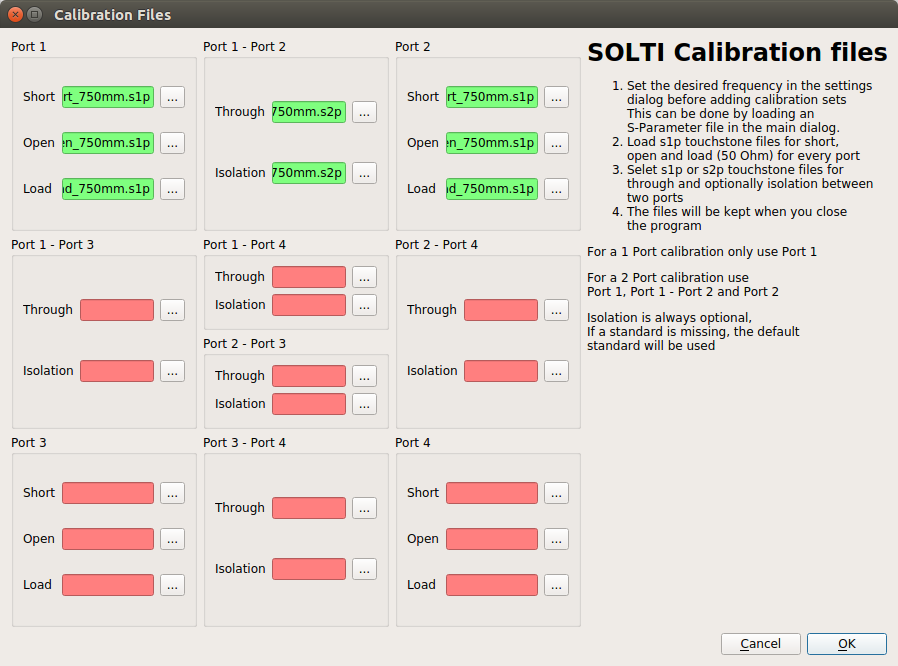
\includegraphics[width=0.75\textwidth]{figures/screenshot3.png}
	\caption{Calibration files dialog}
	\label{fig:caldialog}
\end{figure}
Figure \ref{fig:caldialog} shows the dialog in which the filenames of the measured calibration standards are specified. Depending on the number of ports of the DUT (Device under Test) a number of TouchStone files with measured standards must be supplied. For every port, the following files must be present:
\begin{itemize}
	\item {\textbf{Short:} A measured trace with an uncalibrated network analyzer of the short standard. The file is a one port Touchstone file (.s1p) }
	\item {\textbf{Open:} A measured trace with an uncalibrated network analyzer of the open standard. The file is a one port Touchstone file (.s1p) }
	\item {\textbf{Load:} A measured trace with an uncalibrated network analyzer of the $50\Omega$ load standard. The file is a one port Touchstone file (.s1p) }

\end{itemize}
If the DUT consists of more than one port, also through and optionally isolation standards should be supplied. 
\begin{itemize}
	\item {\textbf{Through:} A measured trace with an uncalibrated network analyzer between the two corresponding ports, with the two cables connected together with a through connector. The file is a two port Touchstone file (.s2p)}
	\item {\textbf{Through:} A measured trace with an uncalibrated network analyzer between the two corresponding ports, with the two cables both connected to a $50\Omega$ load. The file is a two port Touchstone file (.s2p)}
\end{itemize}
The format of the Touchstone files is described in \cite{touchstoneformat}.

If you want to de-embed a two port S-Parameter file, only Short, Open and Load for Port 1 and 2 need to be supplied plus the Through and Isolation between Port 1-2, this calibration set is shown in figure \ref{fig:caldialog}.

If the file supplied with the browse button (...) can be found, the filename colors green, otherwise the box turns red. The green color does not indicate that the file is a valid Touchstone file.

The application DeEmbed comes with some example calibration files, and two DUT files:

The files are located in <installation prefix>/share/examples/ 
\begin{itemize}
\item \textbf{short\_750mm.s1p}: Ideal short simulated with 750mm coaxial cable (qucs)
\item \textbf{open\_750mm.s1p}: Ideal open simulated with 750mm coaxial cable (qucs)
\item \textbf{load\_750mm.s1p}: Ideal $50\Omega$ load simulated with 750mm coaxial cable (qucs)
\item \textbf{through\_750mm.s2p}: Ideal through simulated with 2 times 750mm coaxial cable (qucs)
\item \textbf{isolation\_750mm.s2p}: 2 times 750mm coaxial cable simulated with an open end (qucs)
\item \textbf{dut\_750mm.s2p}: Low pass filter simulated with 2x 750mm coaxial cable (qucs)
\item \textbf{dut\_ideal.s2p}: The same low pass filter simulated without cable

\end{itemize}

If you load the right calibration files (2x short open load and 1x through + isolation) the non-calibrated trace of dut\_ideal will exactly follow the calibrated trace of dut\_750mm. The calibration standards should be chosen as ideal.
\newpage
\subsection{Setting calibration standards}
\label{sec:settingcalstds}

The measured calibration standards described in \ref{sec:loadingcalfiles} are usually not measured with perfect calibration standards, unless a simulator is used to generate the calibration files. In case of a perfect calibration kit, the calibration set ''Ideal''can be used. The equations and the different components in the calibration standards are explained in \ref{sec:calstds}.

\begin{figure}[H]
	\centering
	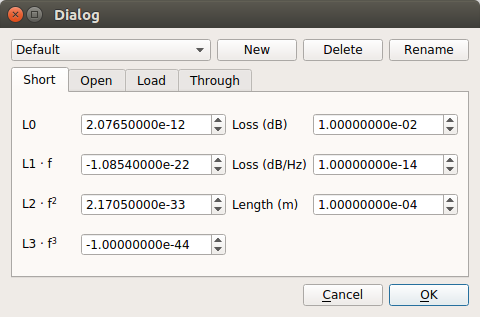
\includegraphics[width=0.75\textwidth]{figures/screenshot4.png}
	\caption{Calibration standards dialog}
	\label{fig:calstddialog}
\end{figure}

An actual calibration kit should come with the different parameters, or the measured calibration kit can be fitted using a simulator to obtain the right standard constants.

A realistic calibration kit (Default) comes with the application, note that this kit does not refer to any commercially available calibration kit.

If you change the calibration standard in this dialog while Touchstone files and calibration files are loaded, the graph will update instantly while changing the constants. This way it is also easy to fit two traces together.
\subsection{Open and save Touchstone files}
From the GUI, Touchstone files can be loaded and saved. DeEmbed handles 1, 2, 3 and 4 port Touchstone files \cite{touchstoneformat}, both to open and save.
\subsection{Navigate the chart}
The chart can be navigated using the mouse wheel and combinations of Shift and Control:
\begin{itemize}
\item    Scrolling zooms the smith chart and centers
\item    Scrolling moves a cartesian chart
\item    Ctrl+scrolling zooms a cartesian chart
\item    Shift+scrolling moves the right cartesian axis
\item    Shift+Ctrl+scrolling zooms the right cartesian axis
\item    A marker can be set by right clicking near to one of the traces.
\end{itemize}
\begin{figure}[H]
	\centering
	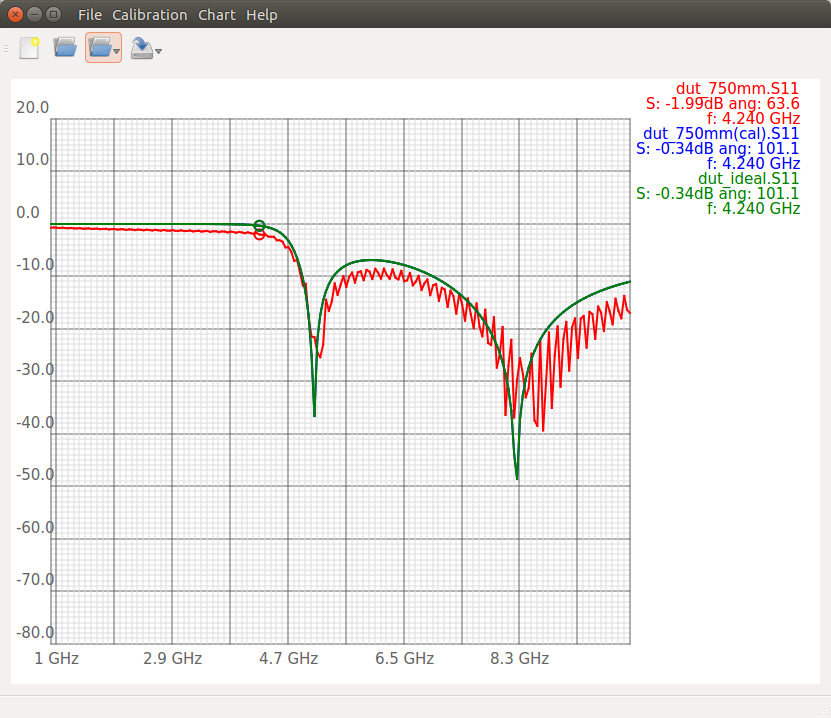
\includegraphics[width=0.75\textwidth]{figures/screenshot2.png}
	\caption{The main window showing the graph in dB mode}
	\label{fig:dbchart}
\end{figure}
\newpage
